\chapter[From Tokens to Training]{From Tokens to Training}
\label{ch:tokens-to-training}

\section{Your Architecture Works. Your Training Doesn't.}

You can write a decoder-only Transformer in a few hundred lines (Chapter~\ref{ch:decoder-only}). You can remove the causal mask and turn it into a bidirectional encoder in ten (Chapter~\ref{ch:bert}). Both architectures are defined by a handful of design choices---attention mask, positional encoding, normalization, activation function---and a competent implementation compiles and runs on the first try.

Then you initialize the weights, feed it text, and the output is random noise.

The architecture has capacity---it \emph{can} represent language. But capacity is not capability. Capability comes from training, and training is where most first attempts fail \emph{silently}. The loss stays flat. The loss explodes to NaN at step 47. The loss decreases beautifully but the generated text is gibberish. The generated text is coherent but the model has memorized its training set verbatim. Each of these failures looks different, but they share a common cause: something in the pipeline between raw text and gradient update is broken, and nothing raised an error.

A correct model plus a broken pipeline is just an expensive random number generator.

This chapter traces the full pipeline that transforms a string of characters into a trained language model. We will follow a single running example---the words \emph{low}, \emph{lower}, \emph{lowest}---from raw text through tokenization, context-window construction, target shifting, loss computation, optimization, and checkpointing. Each stage is a contract between components. Break one contract---feed the wrong token IDs, shift targets incorrectly, skip learning rate warmup, save only model weights without optimizer state---and the pipeline fails, often without telling you.

\begin{quickrecap}
\textbf{What this chapter is and is not.}
\begin{itemize}[nosep,leftmargin=1.5em]
  \item This chapter covers \textbf{single-GPU, small-model training}---everything you need to train a MiniGPT on one machine.
  \item Multi-GPU distributed training, data mixing strategies, and scaling laws are covered in Part~II.
  \item The goal is not to list every hyperparameter, but to explain each stage well enough that you can \emph{diagnose} why a run failed---and know which contract was broken.
\end{itemize}
\end{quickrecap}


\subsection*{Learning Objectives}

After completing this chapter, you should be able to:

\begin{enumerate}
  \item Explain how Byte Pair Encoding (BPE) constructs a subword vocabulary and articulate the vocabulary-size tradeoff.
  \item Describe how tokenized text is chunked into context windows with shifted targets, and identify the silent bugs that arise from getting this wrong.
  \item Trace the training loop: forward pass $\to$ cross-entropy loss $\to$ backward pass $\to$ gradient clipping $\to$ optimizer step $\to$ scheduler step.
  \item Explain why AdamW is the default optimizer for Transformers and why learning rate warmup prevents early-training instability.
  \item Implement checkpointing that saves all necessary state (model, optimizer, scheduler, step count) and correctly resumes training.
\end{enumerate}

\subsection*{Notation}

\begin{center}
\begin{tabular}{ll}
\toprule
Symbol & Meaning \\
\midrule
$V$ & Vocabulary size (number of unique token IDs) \\
$T$ & Context length (tokens per training example) \\
$B$ & Batch size (examples per gradient step) \\
$\eta$ & Learning rate \\
$\beta_1, \beta_2$ & Adam momentum coefficients \\
$\lambda$ & Weight decay coefficient \\
\bottomrule
\end{tabular}
\end{center}

\subsection*{Timeline}

Tokenization and optimization developed largely independently. The key innovations appeared over a decade, but the recipe that modern LLMs use---subword tokenization, adaptive optimization, warmup, and decoupled weight decay---crystallized between 2016 and 2019.

\begin{center}
\begin{tabularx}{\textwidth}{@{}lp{3.8cm}X@{}}
\toprule
Year & Contribution & Key idea \\
\midrule
2015 & Adam~\cite{kingma2015adam} & Adaptive per-parameter learning rates from gradient moments \\
2016 & BPE for NMT~\cite{sennrich2016bpe} & Subword tokenization; merge frequent character pairs \\
2017 & Transformer LR schedule~\cite{vaswani2017attention} & Learning-rate warmup becomes standard for deep attention models \\
2018 & SentencePiece~\cite{kudo2018sentencepiece} & Language-independent tokenization without whitespace assumptions \\
2019 & GPT-2~\cite{radford2019language} & Byte-level BPE; the tokenizer template for GPT-3/4 \\
2019 & AdamW~\cite{loshchilov2019adamw} & Decoupled weight decay; corrects Adam's regularization \\
\bottomrule
\end{tabularx}
\end{center}


%----------------------------------------------------------------------
\section{Text to Tokens: The Contract Between Language and Model}

Every Transformer you have studied so far receives a sequence of integer IDs as input. Chapter~\ref{ch:decoder-only} called these ``tokens'' without explaining where they come from. Chapter~\ref{ch:bert} used \texttt{[CLS]} and \texttt{[MASK]} as if their existence were obvious. Two full chapters of architecture, and the most basic question was never answered: \emph{how does text become numbers?}

A tokenizer is a deterministic algorithm that maps a raw string to a sequence of integers from a fixed vocabulary. It runs before any neural network computation, and its output completely determines what the model sees. The tokenizer decides whether ``New York'' is one token or two, whether ``123456'' splits at the third digit or the fourth, whether a Japanese sentence costs three times as many tokens as its English translation. These decisions are invisible to the model---it never sees the original text---but they shape everything downstream: sequence length, attention cost, what the model can and cannot learn.

This makes the tokenizer one of the most consequential pieces of code in the entire pipeline, and one of the least discussed.

\paragraph{The granularity problem.} There are three natural levels of text decomposition:

\begin{center}
\begin{tabularx}{\textwidth}{@{}l c c X@{}}
\toprule
\textbf{Granularity} & \textbf{Vocab size} & \textbf{Seq.\ length} & \textbf{Problem} \\
\midrule
Character & $\sim$256 & Very long & Sequences become impractically long; $O(T^2)$ attention cost explodes; each character carries little semantic information. \\
Word & $\sim$100K+ & Short & Vocabulary is huge and sparse; unseen words have no representation; morphological variants (run/running/ran) waste separate slots. \\
Subword & $\sim$32K--100K & Moderate & \textbf{Goldilocks:} common words are single tokens; rare words are decomposed into known pieces; vocabulary is compact. \\
\bottomrule
\end{tabularx}
\end{center}

Subword tokenization is the dominant paradigm. GPT-2, GPT-4, LLaMA, and BERT all use variants of it. The core idea: start from characters, iteratively merge frequent pairs into new tokens, and stop when the vocabulary reaches a target size. This is Byte Pair Encoding.

\begin{figure}[ht]
  \centering
  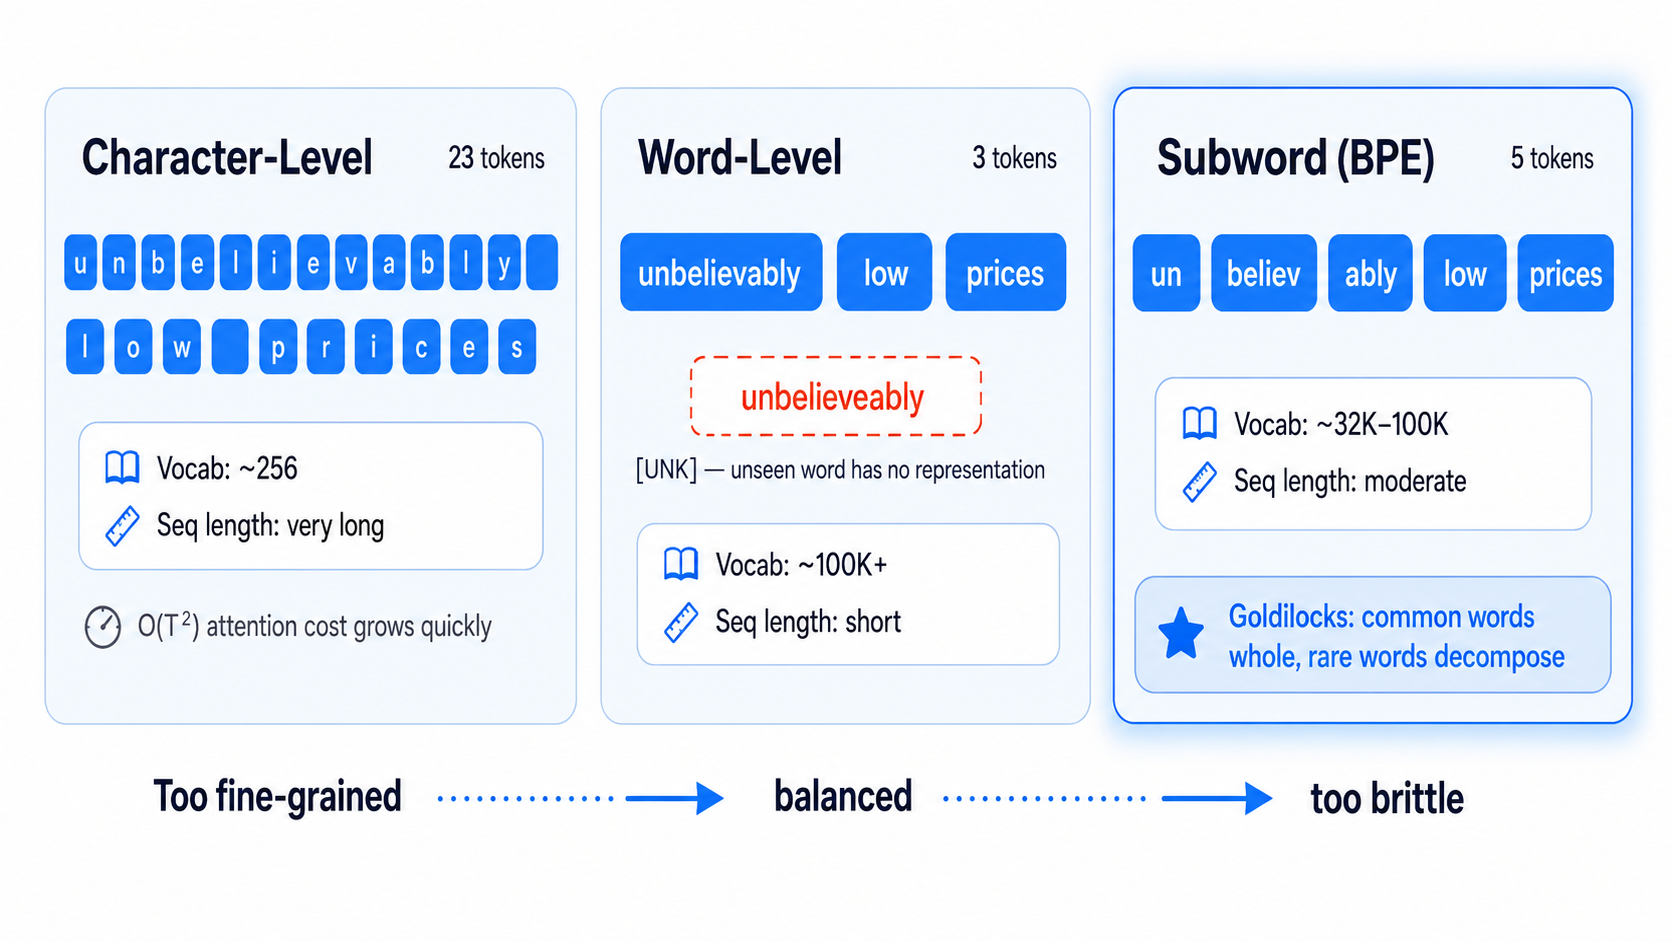
\includegraphics[width=0.85\textwidth]{figures/ch05/granularity_comparison.png}
  \caption{The granularity tradeoff. Character-level tokenization produces long sequences with tiny vocabularies. Word-level tokenization produces short sequences but cannot handle unseen words. Subword tokenization (BPE) is the practical middle ground: common words stay whole, rare words decompose into known subwords.}
  \label{fig:granularity}
\end{figure}

\begin{quickrecap}
\textbf{Quick Recap.}
\begin{itemize}[nosep,leftmargin=1.5em]
  \item A tokenizer converts raw text to integer IDs---it defines the contract between language and model.
  \item Character-level: too long. Word-level: too sparse. Subword: the Goldilocks solution.
  \item The tokenizer runs before any neural computation and silently shapes what the model can learn.
\end{itemize}
\textit{But how does BPE decide which subwords to keep? And what goes wrong when it decides badly?}
\end{quickrecap}


%----------------------------------------------------------------------
\section{BPE, Vocabulary Size, and What Tokenizers Get Wrong}

\paragraph{Byte Pair Encoding: the algorithm.} BPE starts with a character-level vocabulary and iteratively merges the most frequent adjacent pair into a new token. Here is a trace:

\begin{enumerate}[nosep]
  \item \textbf{Initialize:} Treat each character as a token. Corpus: \texttt{["l o w", "l o w e r", "l o w e s t"]}
  \item \textbf{Count pairs:} Most frequent pair is \texttt{(l, o)} --- appears 3 times.
  \item \textbf{Merge:} Replace \texttt{l o} with new token \texttt{lo} everywhere. Now: \texttt{["lo w", "lo w e r", "lo w e s t"]}
  \item \textbf{Repeat:} Next most frequent pair is \texttt{(lo, w)} --- 3 times. Merge to \texttt{low}. Now: \texttt{["low", "low e r", "low e s t"]}
  \item \textbf{Continue} until vocabulary reaches target size $V$.
\end{enumerate}

The merge order is deterministic and saved as a \emph{merge table}. At inference time, the tokenizer applies merges in the same order. The vocabulary size $V$ is a hyperparameter, not learned---you set it before training begins.

\textbf{A subtle point about word boundaries.} Classical BPE (Sennrich et al.) operates \emph{within} pre-tokenized words, not across them---the spaces in the trace above are word boundaries, and merges never cross them. Byte-level BPE (used by GPT-2 and successors) operates on raw bytes and handles word boundaries differently, using special byte encodings for spaces. The distinction matters when you encounter tokenizer outputs like \texttt{\textvisiblespace low} (with a leading space byte): this is not a bug---it is how byte-level BPE represents word-initial tokens.

\begin{figure}[ht]
  \centering
  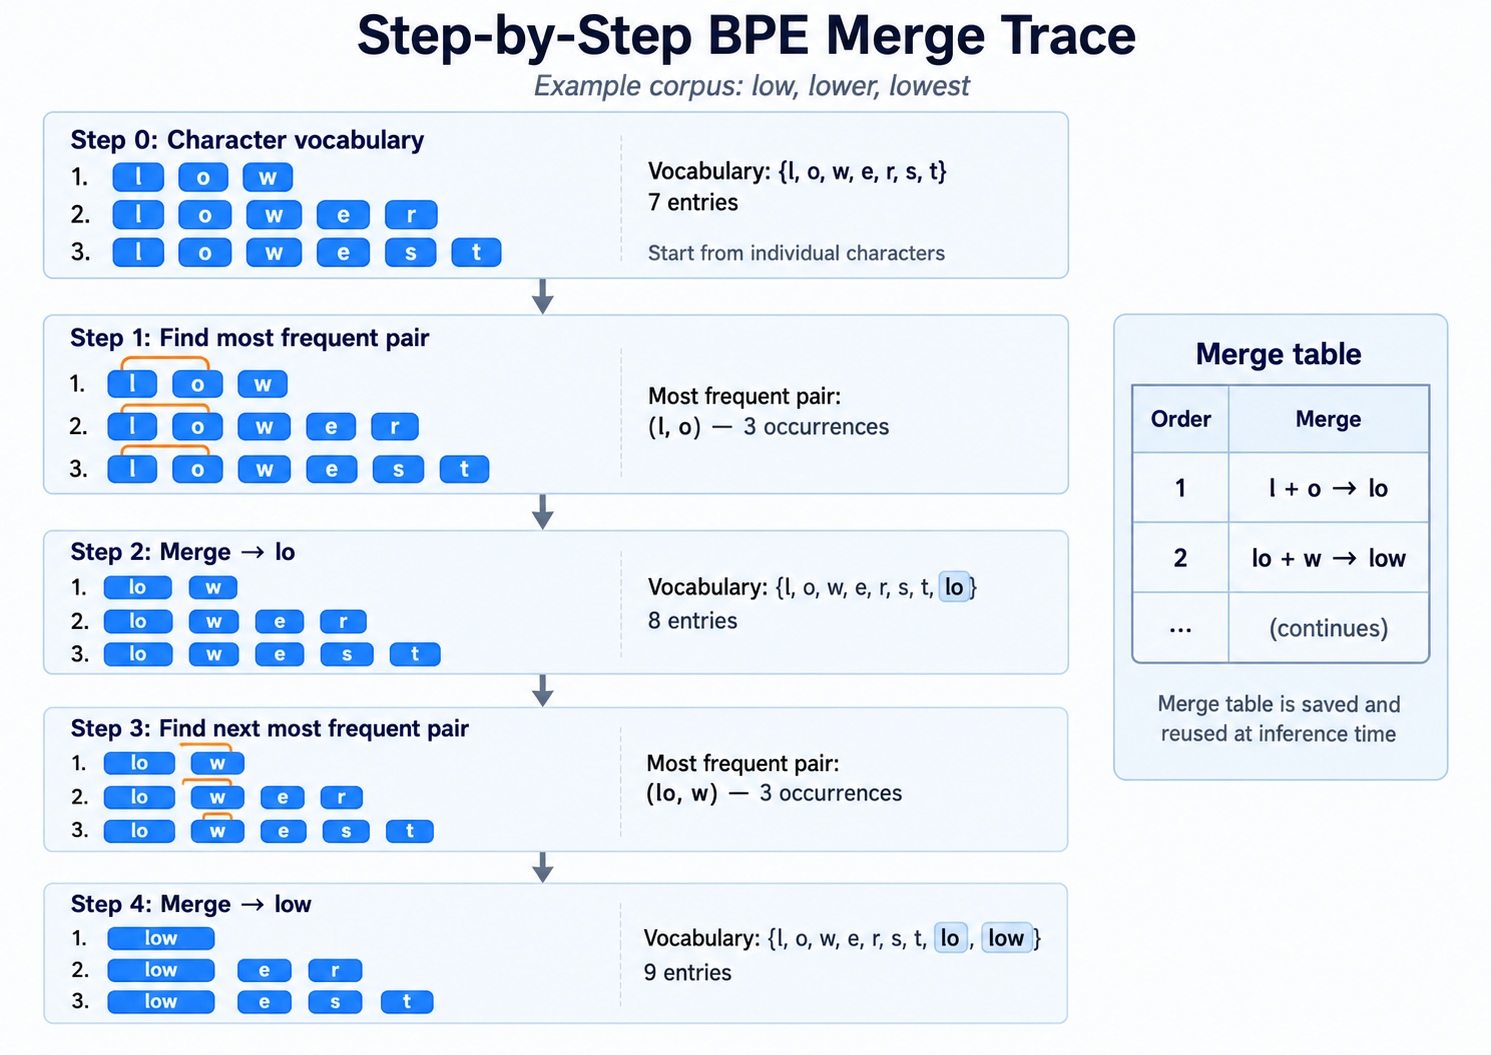
\includegraphics[width=0.85\textwidth]{figures/ch05/bpe_trace.png}
  \caption{Byte Pair Encoding: step-by-step merge trace. Starting from characters, the algorithm merges the most frequent pair at each step. The merge table records the order, and at inference time the same merges are applied to new text.}
  \label{fig:bpe-trace}
\end{figure}

\paragraph{Vocabulary size tradeoff.} Vocabulary size controls the balance between two costs:

\begin{itemize}[nosep]
  \item \textbf{Too small} ($V = 256$, character-level): sequences become very long. A sentence that would be 10 BPE tokens becomes 50+ characters. Longer sequences mean more attention computation and less effective context per window.
  \item \textbf{Too large} ($V = 200K$): the embedding table ($V \times d_{\text{model}}$) becomes enormous. Rare tokens appear infrequently in training data and their embeddings remain poorly trained.
\end{itemize}

In practice, most modern LLMs use $V$ between 32K and 128K. GPT-2 uses 50,257; LLaMA uses 32,000; GPT-4 uses $\sim$100K.

\paragraph{What tokenizers get wrong.} Tokenization introduces silent failure modes that most users never notice:

\textbf{1. Arithmetic failure from token boundaries.} When GPT tokenizes ``$12345 + 67890$'', the numbers may split as \texttt{["123", "45"]} and \texttt{["678", "90"]}---token boundaries do not align with digit boundaries. The model must learn to ``carry'' across token boundaries, which is harder than carrying across digits. This is one reason LLMs struggle with multi-digit arithmetic.

\textbf{2. Multilingual token tax.} BPE vocabularies are trained on data that is predominantly English. Common English words are single tokens, but equivalent phrases in other languages require 3--5$\times$ more tokens. ``Hello'' is 1 token; the Japanese equivalent may be 3--5 tokens. Same meaning, 3--5$\times$ the compute cost, and the effective context window shrinks proportionally.

\begin{figure}[ht]
  \centering
  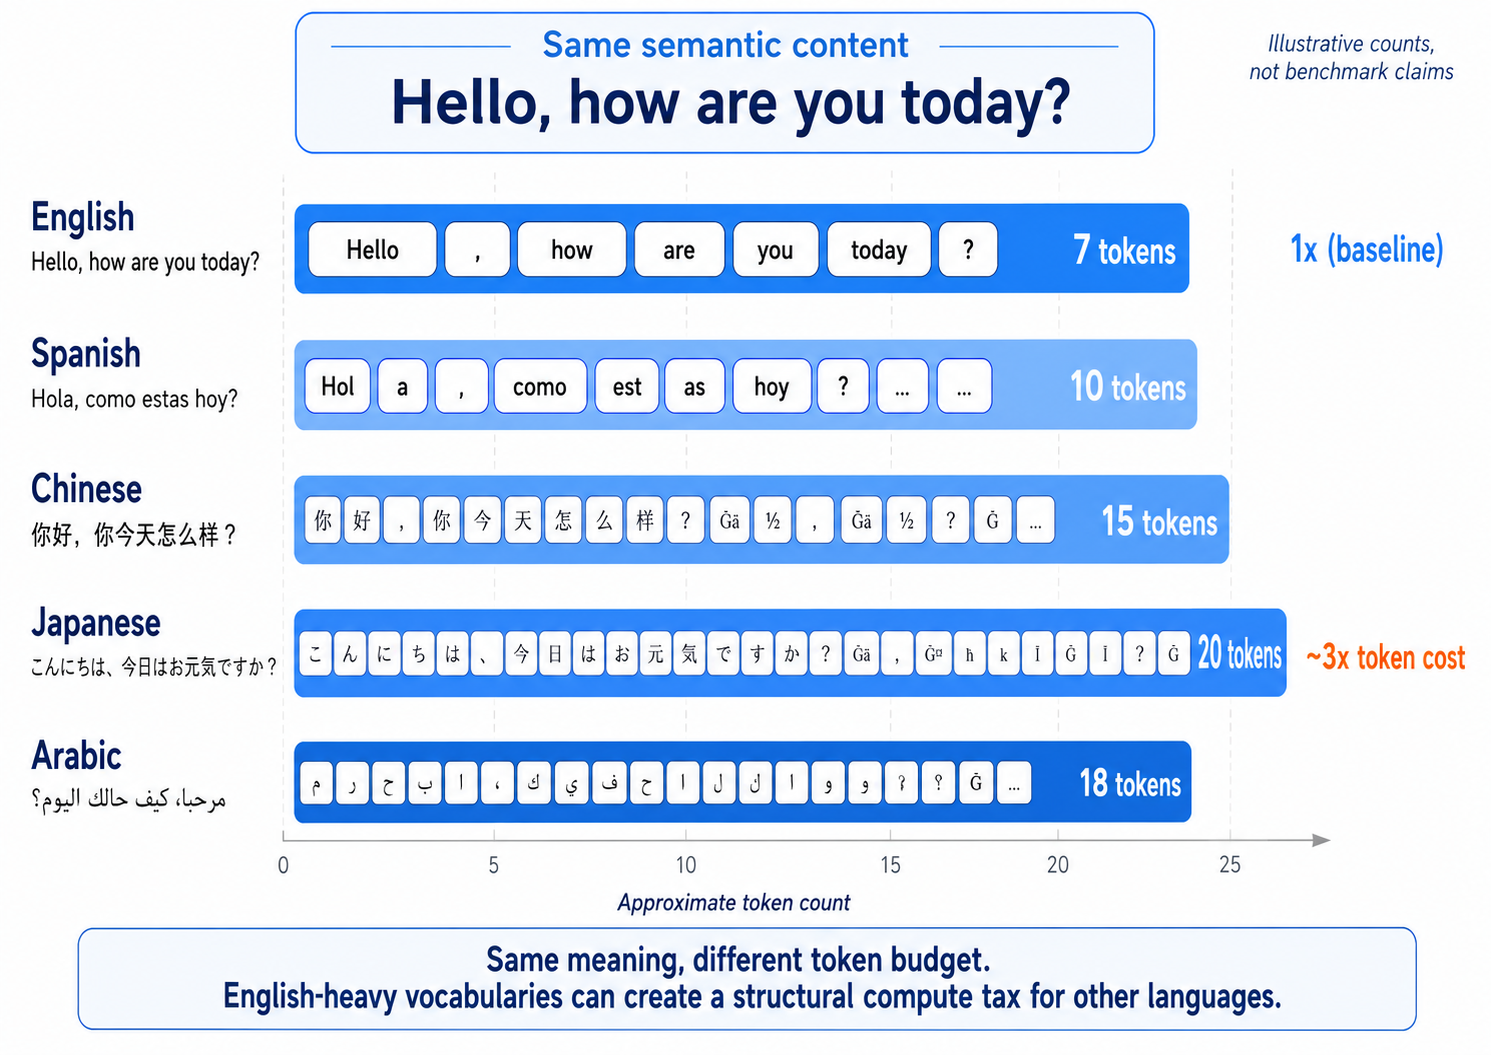
\includegraphics[width=0.85\textwidth]{figures/ch05/multilingual_tokens.png}
  \caption{Multilingual token efficiency. The same semantic content requires dramatically different numbers of tokens across languages. English text is the most efficiently tokenized because most BPE vocabularies are trained primarily on English data.}
  \label{fig:multilingual-tokens}
\end{figure}

\textbf{3. Tokenizer--model coupling.} A model \emph{must} be used with the tokenizer it was trained with. Loading a GPT-2 model with a LLaMA tokenizer produces garbage---every token ID maps to a different word. Special tokens (\texttt{<|endoftext|>}, \texttt{[CLS]}, \texttt{[MASK]}) must exist in the vocabulary. This is not a soft recommendation; it is a hard failure mode.

\begin{center}
\begin{tabularx}{\textwidth}{@{}l X@{}}
\toprule
\textbf{Tokenizer detail} & \textbf{Why it matters} \\
\midrule
Special tokens & Control generation stop, padding, masking \\
Leading spaces & \texttt{" hello"} and \texttt{"hello"} are different tokens---prompt formatting affects behavior \\
Vocab size & Embedding table size vs.\ sequence length tradeoff \\
Byte fallback & Handling unseen Unicode characters without \texttt{[UNK]} \\
\bottomrule
\end{tabularx}
\end{center}

\paragraph{Beyond BPE.} BPE is the most common subword algorithm, but not the only one. WordPiece (used by BERT) selects merges by maximizing likelihood rather than raw frequency. Unigram (used by SentencePiece) starts with a large vocabulary and prunes tokens that contribute least to the likelihood. In practice, the differences in downstream performance are small; the choice is usually determined by framework conventions rather than empirical superiority.

Modern frontier models increasingly use \textbf{byte-level BPE} (GPT-2 onward): the initial vocabulary is the 256 possible bytes rather than Unicode characters. This eliminates the need for Unicode preprocessing and ensures that any input can be tokenized without an \texttt{[UNK]} token.

\fbox{\parbox{0.95\textwidth}{
\textbf{Pause and verify.} Take the string ``unbelievably'' and trace BPE with a small merge table: \texttt{(u,n)$\to$un}, \texttt{(b,e)$\to$be}, \texttt{(l,i)$\to$li}, \texttt{(be,li)$\to$beli}, \texttt{(e,v)$\to$ev}. What tokens result? Now add one more merge: \texttt{(un,beli)$\to$unbeli}. How does the tokenization change? Notice: the merge order determines the final segmentation.
}}

\begin{quickrecap}
\textbf{Quick Recap.}
\begin{itemize}[nosep,leftmargin=1.5em]
  \item BPE builds a vocabulary by iteratively merging frequent character pairs. Vocabulary size is a hyperparameter.
  \item Token boundaries do not respect semantic boundaries---this causes silent failures in arithmetic, code, and multilingual processing.
  \item A model must always be paired with the tokenizer it was trained with. Mismatched tokenizers produce garbage output.
\end{itemize}
\textit{We now have token IDs. But a language model does not train on raw sequences---it trains on carefully shaped windows with shifted targets. Getting this wrong is the quietest catastrophe in deep learning.}
\end{quickrecap}


%----------------------------------------------------------------------
\section{Context Windows and Shifted Targets}

Tokenization converts text to integers. But a raw stream of token IDs is not yet a training example. The model needs two things: an input sequence and a target sequence---and the relationship between them must be exact. This is the most deceptively simple stage of the pipeline, and the one where silent bugs do the most damage.

\paragraph{The shift.} Return to our running example. After BPE, suppose the corpus \emph{``low lower lowest''} becomes the token sequence \texttt{[low, \textvisiblespace low, er, \textvisiblespace low, est]}. With a context length of~5, a single training example looks like this:

\begin{center}
\begin{tabular}{lccccc}
\toprule
& pos 0 & pos 1 & pos 2 & pos 3 & pos 4 \\
\midrule
\textbf{Input}  & \texttt{low} & \texttt{\textvisiblespace low} & \texttt{er} & \texttt{\textvisiblespace low} & --- \\
\textbf{Target} & \texttt{\textvisiblespace low} & \texttt{er} & \texttt{\textvisiblespace low} & \texttt{est} & --- \\
\bottomrule
\end{tabular}
\end{center}

The model sees positions $[0, T{-}1]$ and is asked to predict positions $[1, T]$. Loss is computed at every position. At position~0 the model must predict \texttt{\textvisiblespace low} given only \texttt{low}; at position~2 it must predict \texttt{\textvisiblespace low} given \texttt{[low, \textvisiblespace low, er]}. This is the setup assumed by the cross-entropy loss in the next section.

This training strategy---feeding the ground-truth previous token as input rather than the model's own prediction---is called \textbf{teacher forcing}. At inference time the model must use its own outputs autoregressively, which creates a train/test mismatch (the \emph{exposure bias} problem). For pretraining, teacher forcing is universal: it enables parallel computation across all positions and provides a stable gradient signal.

\textbf{Getting this wrong is a silent bug.} If input and target are identical (no shift), the model can achieve near-zero loss by copying---but it has not learned any language structure. Lab~3 Experiment~0 demonstrated this: unshifted labels produced loss $\approx 0.008$ but completely broken generation. The model's loss looked perfect; its output was garbage.

\paragraph{Chunking a long document.} Training corpora contain documents much longer than the model's context length $T$. There are several strategies for slicing them:

\begin{itemize}[nosep]
  \item \textbf{Non-overlapping chunks.} Slice the token stream into consecutive windows of length $T+1$ (the extra token provides the final target). Simple and fast, but chunk boundaries create hard discontinuities---the first token of each chunk has no left context.
  \item \textbf{Sliding window with stride.} Each window overlaps the previous one by some amount. Reduces boundary artifacts but processes some tokens multiple times, increasing compute cost.
  \item \textbf{Document boundaries.} When chunks span two documents, the model learns to ``continue'' across unrelated texts. Inserting an end-of-document token (\texttt{<eos>}) between documents signals the boundary. Some implementations simply drop chunks that cross document boundaries.
\end{itemize}

For Project~1, non-overlapping chunks with \texttt{<eos>} between documents is the simplest correct approach.

\textbf{Production note: document packing.} At scale, many short documents are \emph{packed} into a single context window to avoid wasting padding tokens. An \texttt{<eos>} token marks each boundary, but this alone is not sufficient: without a modified attention mask, tokens in document~B can attend to tokens in document~A, causing \emph{attention leakage} across unrelated texts. Production implementations reset the causal mask at each document boundary so that attention does not cross the \texttt{<eos>} separator. Project~1 uses a simpler setup (one document per chunk), but you should know that packing-with-attention-masking is standard at frontier scale.

\begin{figure}[ht]
  \centering
  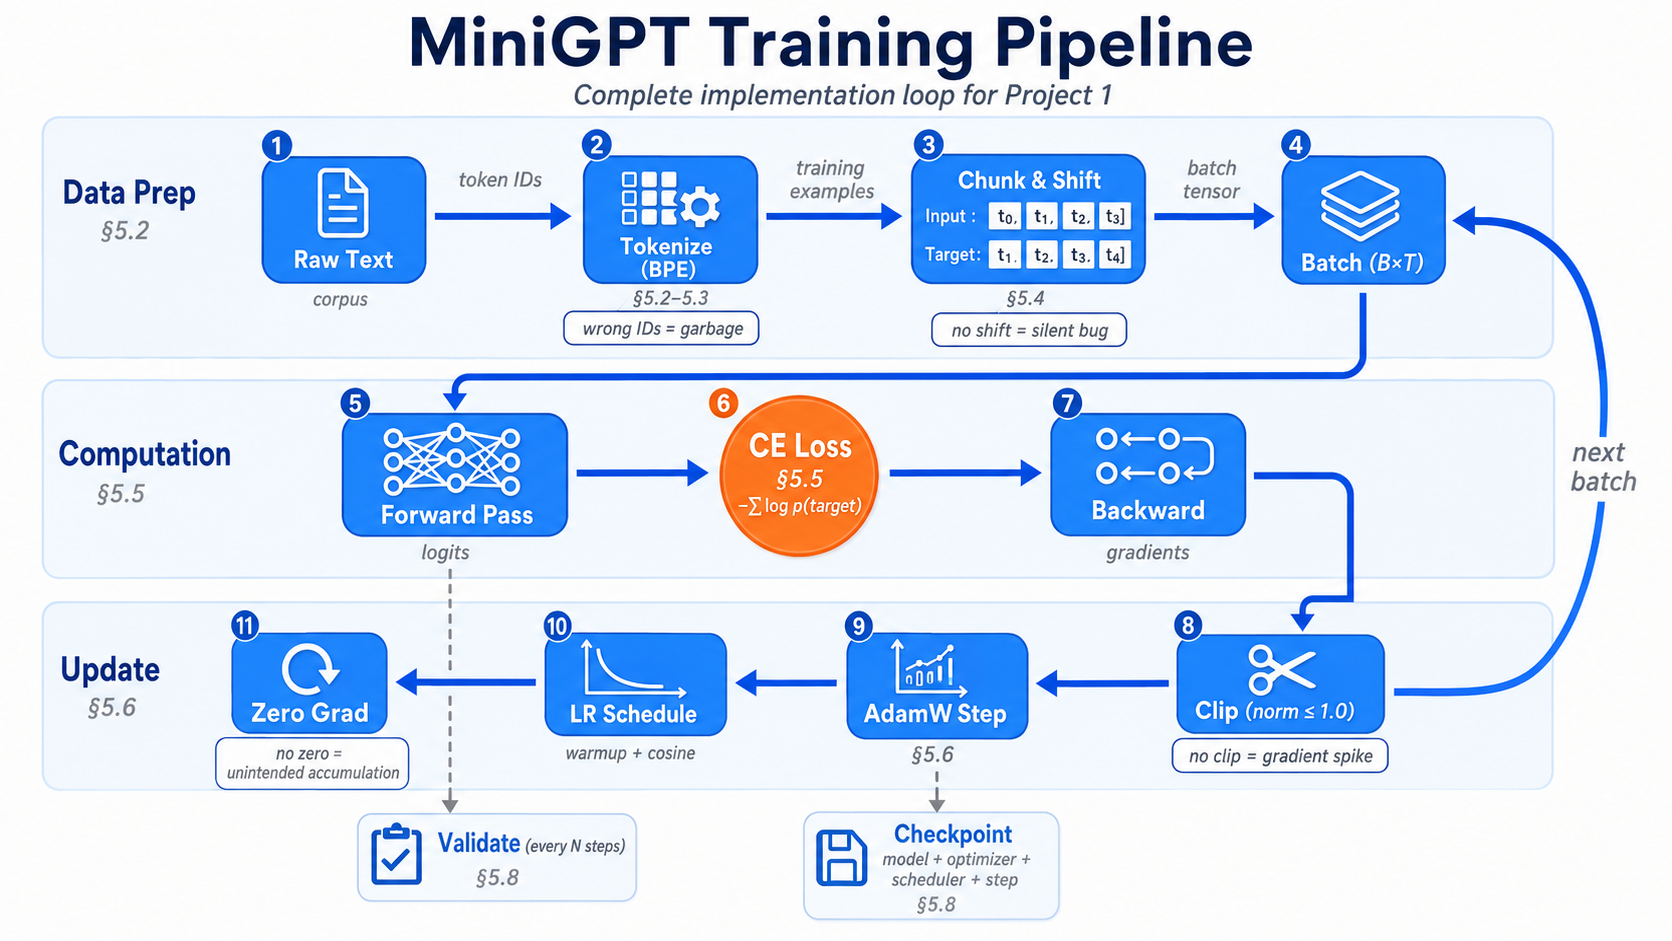
\includegraphics[width=0.9\textwidth]{figures/ch05/training_pipeline.png}
  \caption{The training pipeline from raw text to gradient update. Each stage is a contract: tokenize $\to$ chunk into context windows $\to$ shift targets $\to$ batch $\to$ forward pass $\to$ cross-entropy loss $\to$ backward pass $\to$ clip gradients $\to$ optimizer step $\to$ scheduler step $\to$ validate periodically $\to$ checkpoint. Breaking any contract produces silent failures.}
  \label{fig:training-pipeline}
\end{figure}

\paragraph{Batching and padding.} Training examples are grouped into batches. When sequences in a batch have different lengths, the shorter ones must be padded to the maximum length. Padded positions should be excluded from the loss (typically by setting their target labels to $-100$, which PyTorch's \texttt{CrossEntropyLoss} ignores by default). For fixed-length context windows---the typical setup in language model pretraining---all sequences are the same length and no padding is needed.

\begin{quickrecap}
\textbf{Quick Recap.}
\begin{itemize}[nosep,leftmargin=1.5em]
  \item Training examples are created by shifting the input sequence by one position to create targets.
  \item Long documents are chunked into context-length windows. Non-overlapping chunks with \texttt{<eos>} markers at document boundaries is the simplest correct approach.
  \item Unshifted labels are a silent, catastrophic bug: near-zero loss but broken generation.
\end{itemize}
\textit{Data is shaped. Now: what does the training loop actually do with it, and why do seven lines of code contain so many ways to fail?}
\end{quickrecap}


%----------------------------------------------------------------------
\section{The Next-Token Training Loop}

Our running example has traveled from the raw string \emph{``low lower lowest''} through BPE (\S5.3), context-window chunking, and target shifting (\S5.4). It is now a batch of integer pairs: inputs and targets, one position apart. The model must learn from these pairs. The training loop is deceptively short---seven lines of pseudocode---but each line represents a contract, and violating any one of them will either crash training or produce a model that looks trained but is not:

\begin{lstlisting}[language=Python, caption={Minimal next-token training loop (pseudocode).}]
for batch in dataloader:
    inputs, targets = batch[:, :-1], batch[:, 1:]
    logits = model(inputs)           # (B, T, V)
    loss = cross_entropy(logits.view(-1, V), targets.view(-1))
    loss.backward()
    clip_grad_norm_(model.parameters(), max_norm=1.0)
    optimizer.step()
    scheduler.step()
    optimizer.zero_grad()
\end{lstlisting}

\paragraph{Cross-entropy loss.} The loss answers one question: \emph{at each position, how surprised was the model by the actual next token?}

\[
  \mathcal{L} = -\frac{1}{BT}\sum_{b=1}^{B}\sum_{t=1}^{T} \log p_\theta(x_{b,t} \mid x_{b,<t})
\]

\noindent where $B$ is the batch size and $T$ is the sequence length. The loss averages over all tokens in all sequences in the batch.

Return to our running example. At position~0, the model sees \texttt{low} and must predict \texttt{\textvisiblespace low}. If it assigns $p = 0.4$ to that token, the contribution to the loss at this position is $-\log(0.4) \approx 0.92$. If it assigns $p = 0.01$, the contribution is $-\log(0.01) \approx 4.6$---five times worse. The loss is the average of these surprises across all positions and all sequences in the batch.

The logits (raw outputs of the final linear layer, shape $B \times T \times V$) are converted to probabilities via softmax, but in practice PyTorch's \texttt{CrossEntropyLoss} takes logits directly and applies log-softmax internally for numerical stability.

\textbf{What does the loss number mean?} At initialization, if the model assigns uniform probability over a vocabulary of $V = 50{,}257$ tokens, the expected loss is $\log(V) \approx 10.8$. A well-trained GPT-2 achieves loss $\approx 3.0$ on typical text. In perplexity terms: $e^{10.8} \approx 50{,}000$ (random) vs.\ $e^{3.0} \approx 20$ (trained). Your MiniGPT will start near $\log(V)$ and, if everything in the pipeline is correct, descend steadily from there.

\paragraph{Gradient clipping.} The loss tells the model \emph{what} to fix. But how it fixes it---how the gradient flows backward through the parameters---can itself go wrong. Transformer training is prone to occasional gradient spikes---single batches that produce abnormally large gradients due to rare tokens or unfortunate data combinations. Without clipping, a single spike can permanently damage weights. The function \texttt{clip\_grad\_norm\_} rescales the gradient vector so its global $L_2$ norm does not exceed a threshold (typically 1.0). This is standard for all Transformer training.

\paragraph{The order matters.} In the loop above, the order is: backward $\to$ clip $\to$ step $\to$ scheduler step $\to$ zero grad. Common mistakes:

\begin{itemize}[nosep]
  \item Calling \texttt{optimizer.step()} before \texttt{backward()}: no gradients to apply.
  \item Forgetting \texttt{zero\_grad()}: gradients accumulate across batches (this is intentional in gradient accumulation, but a bug if unintended).
  \item Calling \texttt{scheduler.step()} per epoch instead of per step: warmup and cosine decay happen at the wrong rate.
\end{itemize}

\begin{quickrecap}
\textbf{Quick Recap.}
\begin{itemize}[nosep,leftmargin=1.5em]
  \item Cross-entropy loss measures how well the model predicts the actual next token. At random: $\sim$10.8; well-trained: $\sim$3.0.
  \item Gradient clipping prevents rare spikes from destroying weights. Max norm of 1.0 is standard.
  \item The loop is seven lines, but ordering (backward $\to$ clip $\to$ step $\to$ schedule $\to$ zero\_grad) is critical.
\end{itemize}
\textit{The loop tells the model \emph{how} to update. The optimizer and learning rate schedule determine \emph{how much}---and getting the schedule wrong is the single most common cause of training failure.}
\end{quickrecap}


%----------------------------------------------------------------------
\section{AdamW, Warmup, and Cosine Decay}

\paragraph{Why not SGD?} The loss function tells the model what to learn. The optimizer tells it \emph{how fast} to learn---and for Transformers, the answer is: not at the same speed everywhere. Stochastic gradient descent updates all parameters with the same learning rate. But Transformers have parameters that vary enormously in scale---embedding tables, attention projection matrices, layer norm gains---and a single learning rate is too large for some and too small for others. Adaptive optimizers like Adam maintain \emph{per-parameter} learning rate estimates based on the history of each parameter's gradients.

\paragraph{Adam and AdamW.} Adam~\cite{kingma2015adam} tracks two exponential moving averages for each parameter: the first moment $m_t$ (mean of recent gradients) and the second moment $v_t$ (mean of recent squared gradients). The update divides by $\sqrt{v_t}$, effectively normalizing each parameter's step size by its gradient magnitude.

AdamW~\cite{loshchilov2019adamw} corrects a subtle issue: in the original Adam, weight decay is entangled with the adaptive learning rate. AdamW \emph{decouples} weight decay from the gradient-based update. The full update rule, including bias correction:

\begin{align}
  m_t &= \beta_1 m_{t-1} + (1 - \beta_1) g_t, \qquad
  v_t = \beta_2 v_{t-1} + (1 - \beta_2) g_t^2 \notag \\[4pt]
  \hat{m}_t &= \frac{m_t}{1 - \beta_1^t}, \qquad
  \hat{v}_t = \frac{v_t}{1 - \beta_2^t} \label{eq:bias-correction} \\[4pt]
  \theta_{t+1} &= \theta_t - \eta \left( \frac{\hat{m}_t}{\sqrt{\hat{v}_t} + \epsilon} + \lambda \theta_t \right) \notag
\end{align}

\noindent The bias-correction step (Eq.~\ref{eq:bias-correction}) is essential: at early steps, $m_t$ and $v_t$ are initialized to zero and biased toward small values. Without correction, Adam systematically underestimates the gradient magnitude in the first few hundred steps---a second source of early-training instability alongside the noisy-gradient problem that warmup addresses. Bias correction and warmup are complementary: correction fixes the optimizer's \emph{internal} estimates; warmup limits the optimizer's \emph{external} step size.

The $\lambda \theta_t$ term is the decoupled weight decay---it shrinks weights independently of the adaptive step. In original Adam, weight decay was applied through the gradient, entangling it with the per-parameter scaling. AdamW decouples the two, ensuring that weight decay behaves the same regardless of gradient magnitude. This decoupled formulation is now the default for Transformer training. Typical values: $\beta_1 = 0.9$, $\beta_2 = 0.999$, $\epsilon = 10^{-8}$, $\lambda = 0.01$--$0.1$.

\begin{figure}[ht]
  \centering
  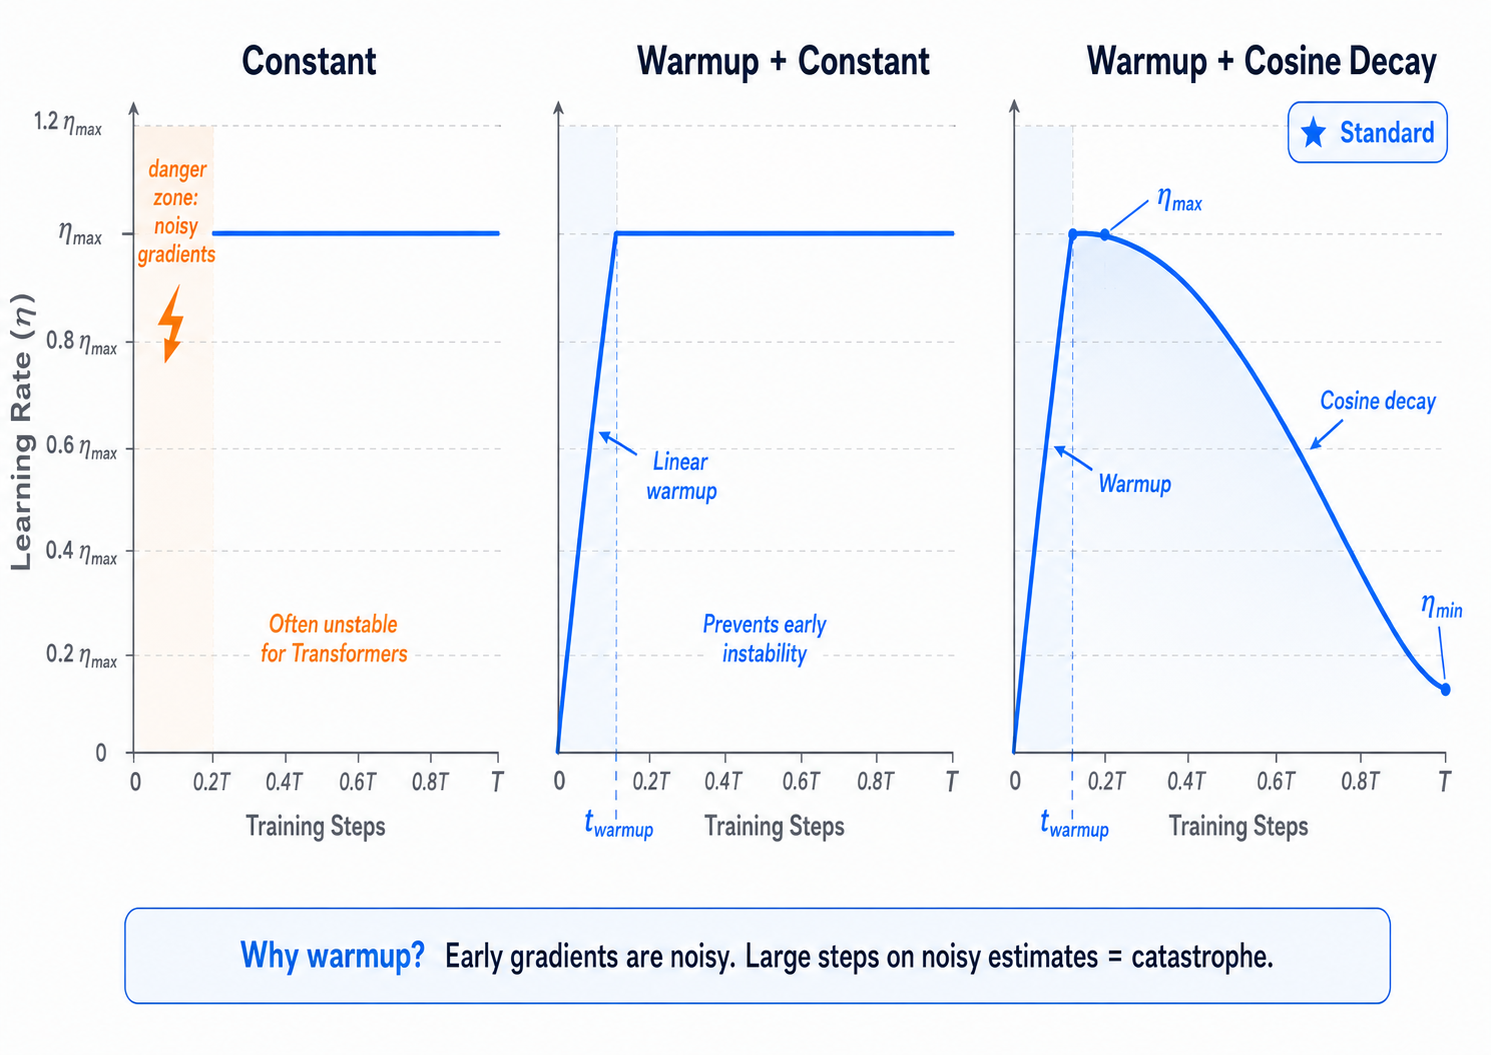
\includegraphics[width=0.85\textwidth]{figures/ch05/lr_schedule.png}
  \caption{Learning rate schedules for Transformer training. \textbf{Left:} constant learning rate---common for convnets but often unstable for Transformers. \textbf{Center:} warmup + constant---linear ramp from zero prevents early instability. \textbf{Right:} warmup + cosine decay---the standard recipe. The learning rate increases linearly during warmup, then follows a cosine curve to near zero.}
  \label{fig:lr-schedule}
\end{figure}

\paragraph{Why warmup?} At the start of training, the model's representations are random. Gradients computed on random features are noisy estimates of the true gradient direction. Taking large steps based on noisy estimates can push parameters into regions from which recovery is difficult---loss spikes or diverges.

Warmup solves this by starting with a very small learning rate and linearly increasing it over the first few hundred to few thousand steps. By the time the learning rate reaches its peak, the model's representations have stabilized enough that the gradients are meaningful.

This connects directly to Chapter~\ref{ch:decoder-only}'s discussion of pre-norm: Pre-LayerNorm controls the \emph{scale} of activations at initialization; warmup controls the \emph{scale} of parameter updates. Both address the same underlying problem: training instability in the first few steps.

\paragraph{Weight initialization: prevention, not just treatment.} Warmup treats early instability from the optimizer side. Proper initialization prevents it from the forward-pass side. GPT-2 scales the initialization of residual-path projections by $1/\sqrt{2N}$, where $N$ is the number of layers:

\[
  W_{\text{residual}} \sim \mathcal{N}\!\left(0,\; \frac{0.02}{\sqrt{2N}}\right)
\]

\noindent Without this scaling, the variance of the residual stream grows with depth at initialization, and the first backward pass produces enormous gradients in the early layers. Embedding layers are typically initialized with $\sigma = 0.02$; LayerNorm gains are initialized to~1 and biases to~0. These are not ``hyperparameters to tune''---they are load-bearing defaults. If your first training run diverges despite warmup and clipping, check initialization before changing the learning rate.

\paragraph{Cosine decay.} After warmup, the learning rate follows a cosine curve from the peak value to near zero. The intuition maps onto what the model is doing at different stages of training: early on, it makes coarse structural adjustments---learning that verbs follow nouns, that punctuation ends sentences, that certain token pairs co-occur. Later, it refines the probability distribution at a much finer grain---getting the relative likelihood of ``happy'' vs.\ ``glad'' right in specific contexts. Large steps in this late phase overshoot these refinements; a decaying learning rate prevents it.

The full schedule:
\[
  \eta(t) = \begin{cases}
    \eta_{\max} \cdot \frac{t}{t_{\text{warmup}}} & \text{if } t < t_{\text{warmup}} \\[6pt]
    \eta_{\min} + \frac{1}{2}(\eta_{\max} - \eta_{\min})\left(1 + \cos\left(\frac{t - t_{\text{warmup}}}{t_{\text{total}} - t_{\text{warmup}}} \cdot \pi\right)\right) & \text{otherwise}
  \end{cases}
\]

Typical values: $\eta_{\max} = 3 \times 10^{-4}$ to $6 \times 10^{-4}$, warmup over 1--5\% of total steps, $\eta_{\min} = 0.1 \times \eta_{\max}$.

\paragraph{Beyond cosine: other schedules.} Cosine decay is the standard recipe for fixed-budget pretraining and the right choice for Project~1. But it has a practical limitation: you must decide the total number of steps \emph{before training begins}, because the cosine curve depends on $t_{\text{total}}$. Two alternatives are worth knowing:

\begin{itemize}[nosep]
  \item \textbf{Inverse square root} (the original Transformer schedule): $\eta(t) \propto 1/\sqrt{t}$ after warmup. Historically important---Vaswani et al.\ used it---but largely superseded by cosine and WSD.
  \item \textbf{WSD (Warmup--Stable--Decay):} warmup to a peak, hold at that peak for most of training, then rapidly decay in a short final phase. Used by DeepSeek, MiniCPM, and several open-source LLMs. The key advantage over cosine: because the learning rate stays at the peak during the stable phase, you can stop training at any point in that phase and either fine-tune or continue pretraining with more data---without wasting a partially completed cosine schedule. For long pretraining runs where the total compute budget may change mid-flight, WSD is increasingly preferred.
\end{itemize}

\fbox{\parbox{0.95\textwidth}{
\textbf{Pause and verify.} You are training a 10M-parameter GPT for 10{,}000 steps with 500 warmup steps and cosine decay. At step 250, what fraction of $\eta_{\max}$ is the learning rate? At step 5{,}000? At step 9{,}500? Sketch the curve on paper before reading on.
}}

\begin{quickrecap}
\textbf{Quick Recap.}
\begin{itemize}[nosep,leftmargin=1.5em]
  \item AdamW is the default optimizer: adaptive per-parameter learning rates with decoupled weight decay.
  \item Warmup prevents early instability by starting with small updates while representations are still random.
  \item Cosine decay gradually reduces the learning rate, allowing fine-grained refinement in late training.
\end{itemize}
\textit{The optimizer decides the step direction; the batch size decides how many examples contribute to each step. What if the batch you need does not fit in GPU memory?}
\end{quickrecap}


%----------------------------------------------------------------------
\section{Gradient Accumulation, Clipping, and Throughput}

\paragraph{The batch size problem.} Every stage of the pipeline so far has been about correctness: the right tokens, the right shift, the right loss, the right optimizer. This section is about \emph{throughput}---how to push more tokens through the pipeline per second without running out of GPU memory.

The tension is simple. Stable gradients require large batches: averaging over more examples smooths out the noise from individual data points. But large batches consume proportionally more memory, and a single consumer GPU often cannot fit more than a handful of examples. Gradient accumulation resolves this: run multiple forward-backward passes, let the gradients accumulate, and only call \texttt{optimizer.step()} after $k$ passes:

\begin{lstlisting}[language=Python, caption={Gradient accumulation.}]
for i, batch in enumerate(dataloader):
    loss = model(batch) / accumulation_steps
    loss.backward()
    if (i + 1) % accumulation_steps == 0:
        clip_grad_norm_(model.parameters(), max_norm=1.0)
        optimizer.step()
        scheduler.step()
        optimizer.zero_grad()
\end{lstlisting}

If the physical batch size is $B_{\text{micro}} = 8$ and \texttt{accumulation\_steps} = 4, the effective batch size is $B_{\text{eff}} = 32$. The loss is divided by \texttt{accumulation\_steps} so that the accumulated gradient has the same scale as a single large-batch gradient.

\paragraph{Mixed precision (sidebar).} Modern GPUs can perform half-precision arithmetic much faster than fp32. Mixed-precision training stores master weights in fp32 but performs forward and backward passes in a 16-bit format, then converts gradients back to fp32 for the optimizer step.

The two 16-bit formats are \emph{not} interchangeable:
\begin{itemize}[nosep]
  \item \textbf{bf16} (bfloat16) has the same exponent range as fp32 (8 exponent bits) but fewer mantissa bits. Because the exponent range matches fp32, gradients and activations rarely overflow or underflow, and \emph{loss scaling is typically unnecessary}. bf16 is the default choice for modern LLM training (LLaMA, GPT-4 class models, DeepSeek).
  \item \textbf{fp16} has a narrower exponent range (5 exponent bits). Small gradients underflow to zero; large activations overflow to \texttt{inf}. To compensate, fp16 training requires \emph{dynamic loss scaling}---multiplying the loss by a large factor before backward, then dividing gradients afterward. fp16 is now largely a legacy choice, used mainly on older hardware (e.g., V100) that lacks bf16 support.
\end{itemize}

\noindent For a MiniGPT with a few million parameters on a single GPU, the speedup from either format is modest---fp32 training is already fast. At scale (billions of parameters, multi-GPU), mixed precision is essential. Project~1 does not require it, but Part~II will revisit this in detail.

\paragraph{Throughput metrics.} Two numbers characterize training speed:

\begin{itemize}[nosep]
  \item \textbf{Tokens per second.} $B_{\text{eff}} \times T / \text{step\_time}$. This is the primary throughput metric.
  \item \textbf{MFU (Model FLOPs Utilization).} Actual FLOPs / theoretical peak FLOPs. Measures how well you are using the hardware. Typical values: 30--50\% for well-optimized single-GPU training.
\end{itemize}

\begin{quickrecap}
\textbf{Quick Recap.}
\begin{itemize}[nosep,leftmargin=1.5em]
  \item Gradient accumulation simulates large batches without requiring more GPU memory.
  \item Mixed precision helps at scale but is optional for small models.
  \item Throughput = tokens/second. MFU tells you how much of the GPU you are actually using.
\end{itemize}
\textit{You can now train a model. But how do you know if training is working? And what must you save so that an interrupted run can continue exactly where it left off?}
\end{quickrecap}


%----------------------------------------------------------------------
\section{Validation, Checkpointing, Resume, and Reproducibility}

\paragraph{Validation.} A falling training loss is not proof that the model is learning well---it might be memorizing the training set. The only reliable signal is \textbf{validation loss}: the model's performance on text it has never seen during training. Evaluate every $N$ steps (not epochs---steps, because language model training often runs for a single epoch or less):

\begin{itemize}[nosep]
  \item \textbf{Train loss $\downarrow$, val loss $\downarrow$:} training is working.
  \item \textbf{Train loss $\downarrow$, val loss flat or $\uparrow$:} overfitting. Stop or increase data.
  \item \textbf{Both flat:} learning rate too small, or the model has saturated on this data size.
  \item \textbf{Both $\uparrow$ or NaN:} learning rate too high, or a data pipeline bug.
\end{itemize}

\paragraph{What to checkpoint.} Saving only model weights is the most common checkpointing mistake. A checkpoint that enables correct resume must include:

\begin{center}
\begin{tabularx}{\textwidth}{@{}l X@{}}
\toprule
\textbf{Component} & \textbf{Why it is needed} \\
\midrule
Model \texttt{state\_dict} & The trained weights \\
Optimizer \texttt{state\_dict} & Adam's momentum and variance estimates ($m_t, v_t$); without these, the optimizer restarts cold \\
Scheduler \texttt{state\_dict} & Current position in the warmup/cosine schedule \\
Step count / epoch & So training resumes from the correct position \\
RNG states & \texttt{torch.random}, \texttt{cuda}, \texttt{numpy}, \texttt{python} random states for exact reproducibility \\
Config / hyperparameters & Model architecture, learning rate, batch size---so the checkpoint is self-documenting \\
\bottomrule
\end{tabularx}
\end{center}

\paragraph{Resume correctness.} After loading a checkpoint, the training curve should continue as if no interruption occurred. If the loss jumps at resume:

\begin{itemize}[nosep]
  \item Missing optimizer state: Adam restarts with zero momentum, causing a transient spike.
  \item Missing scheduler state: learning rate resets to its initial value instead of where it was.
  \item Missing RNG state: different data order may cause a visible (though usually harmless) discontinuity.
\end{itemize}

\paragraph{Reproducibility.} Two runs with the same seed, data, and hyperparameters should produce the same loss curve (up to floating-point non-determinism). To get close:

\begin{lstlisting}[language=Python, caption={Reproducibility setup.}]
import torch, random, numpy as np
seed = 42
torch.manual_seed(seed)
torch.cuda.manual_seed_all(seed)
random.seed(seed)
np.random.seed(seed)
torch.backends.cudnn.deterministic = True
torch.backends.cudnn.benchmark = False
\end{lstlisting}

Note: full determinism on GPU is not always achievable due to non-deterministic operations (e.g., \texttt{atomicAdd} in some CUDA kernels). The goal is ``close enough''---same loss trajectory within noise.

\begin{quickrecap}
\textbf{Quick Recap.}
\begin{itemize}[nosep,leftmargin=1.5em]
  \item Validate every $N$ steps. Watch for train/val divergence as the overfitting signal.
  \item Checkpoints must include model, optimizer, scheduler, step count, and RNG states.
  \item A correct resume produces a continuous loss curve. Jumps at resume indicate missing state.
\end{itemize}
\textit{Every stage of the pipeline can fail silently. The next section catalogs these failures---organized by source---so you know where to look when your first MiniGPT run goes wrong.}
\end{quickrecap}


%----------------------------------------------------------------------
\section{Failure Modes in MiniGPT Training}
\label{sec:training-failures}

When your first MiniGPT run goes wrong---and it will---the symptom alone rarely tells you the cause. ``Loss is NaN'' could be a learning rate problem, a data pipeline problem, or a numerical stability problem. ``Loss looks great'' could mean the model is learning, or it could mean the targets are unshifted and the model is cheating.

The failures below are organized by \emph{source}, not by symptom. Each entry includes the symptom you will see, the underlying cause, and how to diagnose it. When something breaks, start from the top of the relevant category and work down.

\paragraph{Tokenization failures.}

\begin{itemize}
  \item \textbf{Mismatched tokenizer.} \emph{Symptom:} loss decreases, but generation is gibberish.
  \emph{Cause:} model and tokenizer have different vocabularies, so every token ID maps to the wrong word.
  \emph{Diagnosis:} decode a sample batch back to text and visually inspect.
  \item \textbf{Missing end-of-document tokens.} \emph{Symptom:} generated text is mostly coherent but periodically switches topic mid-sentence.
  \emph{Cause:} without \texttt{<eos>} markers between documents, the model treats cross-document continuation as normal.
  \emph{Diagnosis:} inspect the training data---are document boundaries visible?
  \item \textbf{Number/code boundary misalignment.} \emph{Symptom:} the model fails at multi-digit arithmetic or corrupts code identifiers, even when general text generation is fine. \emph{Cause:} BPE splits numbers and identifiers at arbitrary positions. This is not a bug---it is a known limitation. Be aware when evaluating arithmetic or code generation tasks.
\end{itemize}

\paragraph{Data pipeline failures.}

\begin{itemize}
  \item \textbf{Unshifted labels.} \emph{Symptom:} loss drops to near zero in the first few batches---suspiciously fast. Generation produces repeated tokens or copies of the input. \emph{Cause:} input and target are the same sequence; the model is copying, not predicting. Lab~3 Experiment~0 diagnosed this failure in detail. \emph{Diagnosis:} print \texttt{input[0]} and \texttt{target[0]}. If they are identical, the shift is missing.
  \item \textbf{Padding not masked in loss.} \emph{Symptom:} loss is lower than expected, and the model generates padding tokens during inference. \emph{Cause:} padded positions contribute to the loss, so the model learns that predicting \texttt{<pad>} is rewarding. \emph{Diagnosis:} check that padding targets are set to $-100$.
  \item \textbf{Truncation without chunking.} \emph{Symptom:} training metrics look reasonable but the model seems to have a limited vocabulary and narrow topic range. \emph{Cause:} long documents are truncated to the context window, so the model never sees their tails. If most documents are longer than $T$, a large fraction of tokens are wasted.
\end{itemize}

\paragraph{Training stability failures.}

\begin{itemize}
  \item \textbf{No warmup.} \emph{Symptom:} loss spikes or diverges in the first 50--200 steps, then may or may not recover. \emph{Cause:} early gradients are noisy estimates computed on random features; large steps on noisy estimates push parameters into regions from which recovery is difficult. \emph{Fix:} add warmup over 1--5\% of total steps.
  \item \textbf{Learning rate too high.} \emph{Symptom:} loss explodes to NaN or \texttt{inf} within a few hundred steps. \emph{Cause:} parameter updates overshoot consistently. \emph{Fix:} reduce by 2--5$\times$ and retry.
  \item \textbf{No gradient clipping.} \emph{Symptom:} training is smooth for hundreds or thousands of steps, then the loss suddenly jumps to a much higher value and never recovers. \emph{Cause:} a single batch with abnormally large gradients permanently damages the weights. \emph{Fix:} add \texttt{clip\_grad\_norm\_} with \texttt{max\_norm=1.0}.
  \item \textbf{Unscaled accumulation loss.} \emph{Symptom:} divergence that looks like ``learning rate too high'' but only appears when gradient accumulation is enabled. \emph{Cause:} the loss was not divided by \texttt{accumulation\_steps}, so the effective learning rate is multiplied by that factor. \emph{Fix:} divide the loss by the number of accumulation steps before \texttt{backward()}.
\end{itemize}

\paragraph{Checkpoint/resume failures.}

\begin{itemize}
  \item \textbf{Only saving model weights.} \emph{Symptom:} loss spikes immediately after resume and takes hundreds of steps to recover. \emph{Cause:} Adam's momentum and variance estimates ($m_t, v_t$) are lost; the optimizer restarts cold and must re-estimate them from scratch. \emph{Fix:} save the full \texttt{optimizer.state\_dict()}.
  \item \textbf{Scheduler not restored.} \emph{Symptom:} the learning rate curve has a visible discontinuity at the resume point---typically a sudden jump back to the warmup value. \emph{Cause:} the scheduler restarts from step~0 instead of the saved step. If warmup is short, this triggers a second instability event. \emph{Fix:} save and restore \texttt{scheduler.state\_dict()}.
\end{itemize}


%----------------------------------------------------------------------
\section{Trick Table}

\noindent
\begin{tabularx}{\textwidth}{@{}>{\raggedright\arraybackslash}p{2.8cm}
                              >{\raggedright\arraybackslash}p{2.8cm}
                              >{\raggedright\arraybackslash}p{3.2cm}
                              X@{}}
\toprule
\textbf{Trick} & \textbf{When to use} & \textbf{Expected effect} & \textbf{Failure signal} \\
\midrule
LR warmup &
  Always &
  Prevents early training instability by starting with small steps &
  Loss spikes or NaN in the first 100--500 steps \\[4pt]
Cosine decay &
  Standard for pretraining &
  Smooth learning rate reduction for fine-grained late-stage refinement &
  Loss plateau in late training; model oscillates around minimum \\[4pt]
Gradient clipping &
  Always (\texttt{max\_norm=1.0}) &
  Prevents occasional gradient spikes from destroying weights &
  Sudden, permanent loss jump after many steps of smooth training \\[4pt]
Gradient accumulation &
  When effective batch size exceeds GPU memory &
  Simulates larger batch without more memory &
  Loss diverges if you forget to divide by accumulation steps \\[4pt]
Full checkpoint &
  Every $N$ steps &
  Enables correct resume without loss discontinuity &
  Loss spike at resume point; learning rate visibly wrong \\
\bottomrule
\end{tabularx}


\begin{takeaways}
\begin{itemize}[leftmargin=1.2em, itemsep=4pt]
  \item \textbf{Tokenization is a model interface}, not preprocessing. BPE builds a subword vocabulary by iteratively merging frequent pairs. Vocabulary size, token boundaries, and special tokens silently shape what the model can learn.
  \item Training examples are created by \textbf{shifting the input sequence by one position} to create targets. Unshifted labels are a silent, catastrophic bug.
  \item The next-token \textbf{cross-entropy loss} measures prediction quality at every position, averaged over the batch: $\mathcal{L} = -\frac{1}{BT}\sum_{b,t} \log p(x_{b,t} \mid x_{b,<t})$.
  \item \textbf{AdamW with warmup and cosine decay} is the standard optimizer recipe. Bias correction fixes early-step estimation error; warmup limits step size while representations are random; cosine decay enables fine-grained refinement. Proper weight initialization ($\sigma \propto 1/\sqrt{2N}$ for residual projections) prevents instability from the forward-pass side.
  \item \textbf{Gradient clipping} (max norm 1.0) prevents rare gradient spikes from permanently damaging weights.
  \item A checkpoint must include model, optimizer, scheduler, step count, and RNG states. Missing any component causes discontinuity at resume.
  \item Training failures are diagnostic: each symptom (NaN loss, flat loss, loss spike at resume, good loss but bad generation) maps to a specific pipeline contract violation.
\end{itemize}
\end{takeaways}


\section*{Lab 5: Training Pipeline Diagnostics}

\subsection*{Goal}

Labs~2--4 diagnosed models. Lab~5 diagnoses the \textbf{training pipeline}. You are given a working MiniGPT (the model from Lab~3) and a training script. Your task is not to build a model---it is to observe how pipeline choices change training behavior.

\subsection*{Expected Time}

Core (Experiments~0--2): 2--3 hours. Experiment~3 is shorter but requires careful file handling.

\subsection*{Setup}

See \texttt{labs/ch05/README.md}. You will use the MiniGPT architecture from Lab~3 and train it on a small text corpus (Tiny Shakespeare or similar). All experiments modify the training pipeline, not the model.

\subsection*{Experiment 0: Character vs.\ BPE Tokenization}

\textbf{Corresponds to:} \S5.2--5.3.

\textbf{Goal:} Show that tokenizer choice changes sequence length, training efficiency, and convergence speed.

\begin{enumerate}[nosep]
    \item Train the same MiniGPT architecture on the same corpus, once with character-level tokenization ($V \approx 65$) and once with BPE ($V = 1000$).
    \item Compare: tokens per document, training tokens per second, validation bits-per-byte, and generated samples.
\end{enumerate}

\textbf{Important metric note:} raw cross-entropy loss is not directly comparable across tokenizers. A character model and a BPE model predict different units from different vocabulary sizes. Use raw loss only within a single tokenizer run; for cross-tokenizer comparisons, use a normalized metric such as bits-per-byte (or bytes-per-token plus generation quality).

\textbf{What to look for:} BPE should produce shorter sequences and cover more original text per context window. Character tokenization has a tiny vocabulary but much longer sequences. The result is not ``BPE always has lower raw loss''; the result is that tokenizer choice changes the training problem itself.

\subsection*{Experiment 1: Learning Rate Schedule Ablation (Centerpiece)}

\textbf{Corresponds to:} \S5.6.

\textbf{Goal:} Demonstrate that the learning rate schedule---not just the peak learning rate---determines whether training succeeds.

Run three training configurations with identical architecture and data:

\begin{enumerate}[nosep]
    \item \textbf{No warmup, constant LR} ($\eta = 3 \times 10^{-4}$): expect early instability.
    \item \textbf{Too-high constant LR} ($\eta = 3 \times 10^{-3}$): expect divergence or NaN.
    \item \textbf{Warmup + cosine decay} ($\eta_{\max} = 3 \times 10^{-4}$, 100 warmup steps): expect smooth training.
\end{enumerate}

\textbf{Key deliverable:} One plot with three loss curves. This is the centerpiece figure of Lab~5---it should make the importance of learning rate scheduling immediately visible.

\subsection*{Experiment 2: Vocabulary Size Sweep}

\textbf{Corresponds to:} \S5.3.

\textbf{Goal:} Map the vocabulary-size tradeoff empirically.

\begin{enumerate}[nosep]
    \item Train BPE tokenizers with $V \in \{256, 1000, 4000, 8000\}$ on the same corpus.
    \item Train the same MiniGPT with each tokenizer (same number of gradient steps).
    \item Compare: average sequence length, bytes-per-token, tokens per second, validation bits-per-byte, and sample quality.
\end{enumerate}

\textbf{What to look for:} Very small vocab $\to$ long sequences and less text covered per context window. Very large vocab $\to$ sparse embeddings, with many rare tokens poorly trained on a small corpus. The sweet spot depends on corpus size and model size. Do not rank vocabularies by raw per-token loss alone; normalize by original text length.

\subsection*{Experiment 3: Checkpoint and Resume}

\textbf{Corresponds to:} \S5.8.

\textbf{Goal:} Verify that your checkpoint captures all necessary state.

\begin{enumerate}[nosep]
    \item Train for 500 steps. Save a full checkpoint (model + optimizer + scheduler + step + RNG).
    \item Resume from the checkpoint and train for 500 more steps.
    \item Run an uninterrupted 1000-step training as reference.
    \item Overlay the resumed loss curve on the uninterrupted curve.
\end{enumerate}

\textbf{What to look for:} The resumed curve should continue smoothly from step 500 with no visible discontinuity. If there is a spike, identify which state component is missing.

\subsection*{Report Question}

\begin{quote}
Chapter~5 argues that a correct architecture is necessary but not sufficient---the training pipeline must be aligned end-to-end. Using your Lab~5 experiments: (a) how does tokenizer choice affect training efficiency? (b) what happens when the learning rate schedule is wrong, and why? (c) what must a checkpoint contain for correct resume?
\end{quote}


\section{Summary}

\paragraph{What this chapter built.} Chapters~\ref{ch:decoder-only} and~\ref{ch:bert} gave you two architectures---one that generates, one that represents. This chapter gave you the machinery that turns either one from a randomly initialized function into something that understands language. We traced a single path---from the string \emph{``low lower lowest''} through BPE merges, context-window chunking, shifted targets, cross-entropy loss, AdamW updates, and checkpointed state---and at every stage we asked the same question: \emph{what breaks if this contract is violated?}

\paragraph{The pipeline contract.} The lesson is not any single technique. It is that a trained language model is not a model---it is a \emph{system}. A tokenizer that determines the input vocabulary. A data pipeline that shapes training examples. A loss function that defines the learning signal. An optimizer that updates weights stably. A checkpoint that preserves all state. These five components form a contract. Break one term---feed the wrong token IDs, skip the target shift, forget warmup, save only model weights---and the system fails. Usually silently.

\paragraph{Diagnostic, not prescriptive.} This chapter did not give you ``the best'' hyperparameters. It gave you something more durable: the ability to \emph{diagnose} why a run failed. NaN loss? Check warmup and clipping. Good loss but bad generation? Check the target shift. Loss spike at resume? Check optimizer state. Each symptom points to a specific broken contract---and now you know where to look.

\medskip
\noindent\textit{Self-check: Can you trace a BPE merge? Can you explain why AdamW decouples weight decay? Can you list what a checkpoint must contain? Can you diagnose ``loss is near zero but generation is broken''? If any answer is unclear, re-read the corresponding section before moving to Project~1.}

\medskip
\noindent\textbf{What's next.}\quad You now have everything you need to train a small language model from scratch. Project~1 asks you to do exactly that: implement a MiniGPT, train it on a text corpus, analyze tokenizer effects, and diagnose training stability. After that, Part~II scales these ideas to large corpora, distributed systems, and the engineering required to pretrain frontier models.


\section*{Key Equations at a Glance}

\begin{center}
\renewcommand{\arraystretch}{1.6}
\begin{tabularx}{\textwidth}{@{}lX@{}}
\toprule
Component & Equation \\
\midrule
Next-token loss & $\mathcal{L} = -\frac{1}{BT}\sum_{b,t} \log p_\theta(x_{b,t} \mid x_{b,<t})$ \\[4pt]
Initial loss (random) & $\mathcal{L}_0 = \log V$ \quad ($\approx 10.8$ for $V = 50{,}257$) \\[4pt]
Bias correction & $\hat{m}_t = m_t/(1-\beta_1^t)$, \quad $\hat{v}_t = v_t/(1-\beta_2^t)$ \\[4pt]
AdamW update & $\theta_{t+1} = \theta_t - \eta \left(\frac{\hat{m}_t}{\sqrt{\hat{v}_t} + \epsilon} + \lambda \theta_t\right)$ \\[4pt]
Residual init scale & $W_{\text{res}} \sim \mathcal{N}(0,\; 0.02/\sqrt{2N})$ \\[4pt]
Cosine LR schedule & $\eta(t) = \eta_{\min} + \tfrac{1}{2}(\eta_{\max} - \eta_{\min})(1 + \cos(\pi \cdot \text{progress}))$ \\[4pt]
Effective batch size & $B_{\text{eff}} = B_{\text{micro}} \times \text{accumulation\_steps}$ \\
\bottomrule
\end{tabularx}
\end{center}


\section*{Key Readings}

\begin{enumerate}
  \item \textbf{Sennrich et al., ``Neural Machine Translation of Rare Words with Subword Units'' (2016)}~\cite{sennrich2016bpe}. The paper that introduced BPE to NLP. Focus on: the merge algorithm, the vocabulary size tradeoff, and how subwords handle unseen words.

  \item \textbf{Kingma \& Ba, ``Adam: A Method for Stochastic Optimization'' (2015)}~\cite{kingma2015adam}. The Adam optimizer paper. Focus on: the first and second moment estimates, bias correction, and why adaptive learning rates help with non-stationary objectives.

  \item \textbf{Loshchilov \& Hutter, ``Decoupled Weight Decay Regularization'' (2019)}~\cite{loshchilov2019adamw}. Why weight decay should be decoupled from the adaptive gradient. Short paper; the core insight is in Sections 2--3.

  \item \textbf{Kudo \& Richardson, ``SentencePiece: A simple and language independent subword tokenizer and detokenizer'' (2018)}~\cite{kudo2018sentencepiece}. The tokenizer framework used by LLaMA, T5, and many multilingual models. Focus on: why language-independent tokenization matters.

  \item \textbf{Radford et al., ``Language Models are Unsupervised Multitask Learners'' (GPT-2, 2019)}~\cite{radford2019language}. Section 2 describes the byte-level BPE tokenizer that became the template for GPT-3 and GPT-4. Also demonstrates that next-token prediction on enough data produces a surprisingly capable model.

  \item \textbf{Xiong et al., ``On Layer Normalization in the Transformer Architecture'' (2020)}~\cite{xiong2020layernorm}. Analyzes why Pre-LN Transformers are easier to train and require less warmup than Post-LN. Connects directly to this chapter's discussion of warmup and Chapter~\ref{ch:decoder-only}'s discussion of pre-norm.
\end{enumerate}
